\chapter{Een chemisch systeem beschrijven: voortgang, activiteiten, Q en K}\label{ch:b1:extent-q-and-k}

Een waterstoffabriek voert aardgas en stoom in buizen die roodgloeiend
verhit worden; wat eruit komt, is nooit zuivere waterstof maar een mengsel
van waterstof, koolstofmonoxide, koolstofdioxide, niet-omgezet methaan en
stoom, waarvan de ingenieurs de verhoudingen moeten kennen voordat ze de
volgende eenheid ontwerpen. De samenstelling voorspellen die een reactor
verlaat --- de eindtoestand van een chemisch systeem --- is het onderwerp
van dit hoofdstuk. Daarvoor zijn nodig: een nauwkeurige beschrijving van
het systeem (zijn grootheden en zijn samenstelling), één enkel getal dat
meet hoe ver een reactie gevorderd is (de voortgang), en de wet die zegt
waar de reactie stopt (de evenwichtsconstante). Deze werktuigen worden in
elk later hoofdstuk over oplossingen gebruikt.

\begin{recall}
Boek 1 (jaar 10) volgde een reactie met een voortgangstabel en vond de
\omterm{def:b1:extent-q-and-k:max-extent}{beperkende beginstof}; Boek 1 (jaar 12) voerde het \omterm{def:b1:extent-q-and-k:quotient}{reactiequotiënt} $Q$ en
de evenwichtsconstante $K$ van een niet-aflopende reactie in. Uit de
natuurkunde gebruiken we de ideale gaswet $pV = nRT$, met $R =
\qty{8.314}{J/(mol.K)}$.
\end{recall}

\begin{omfigure}
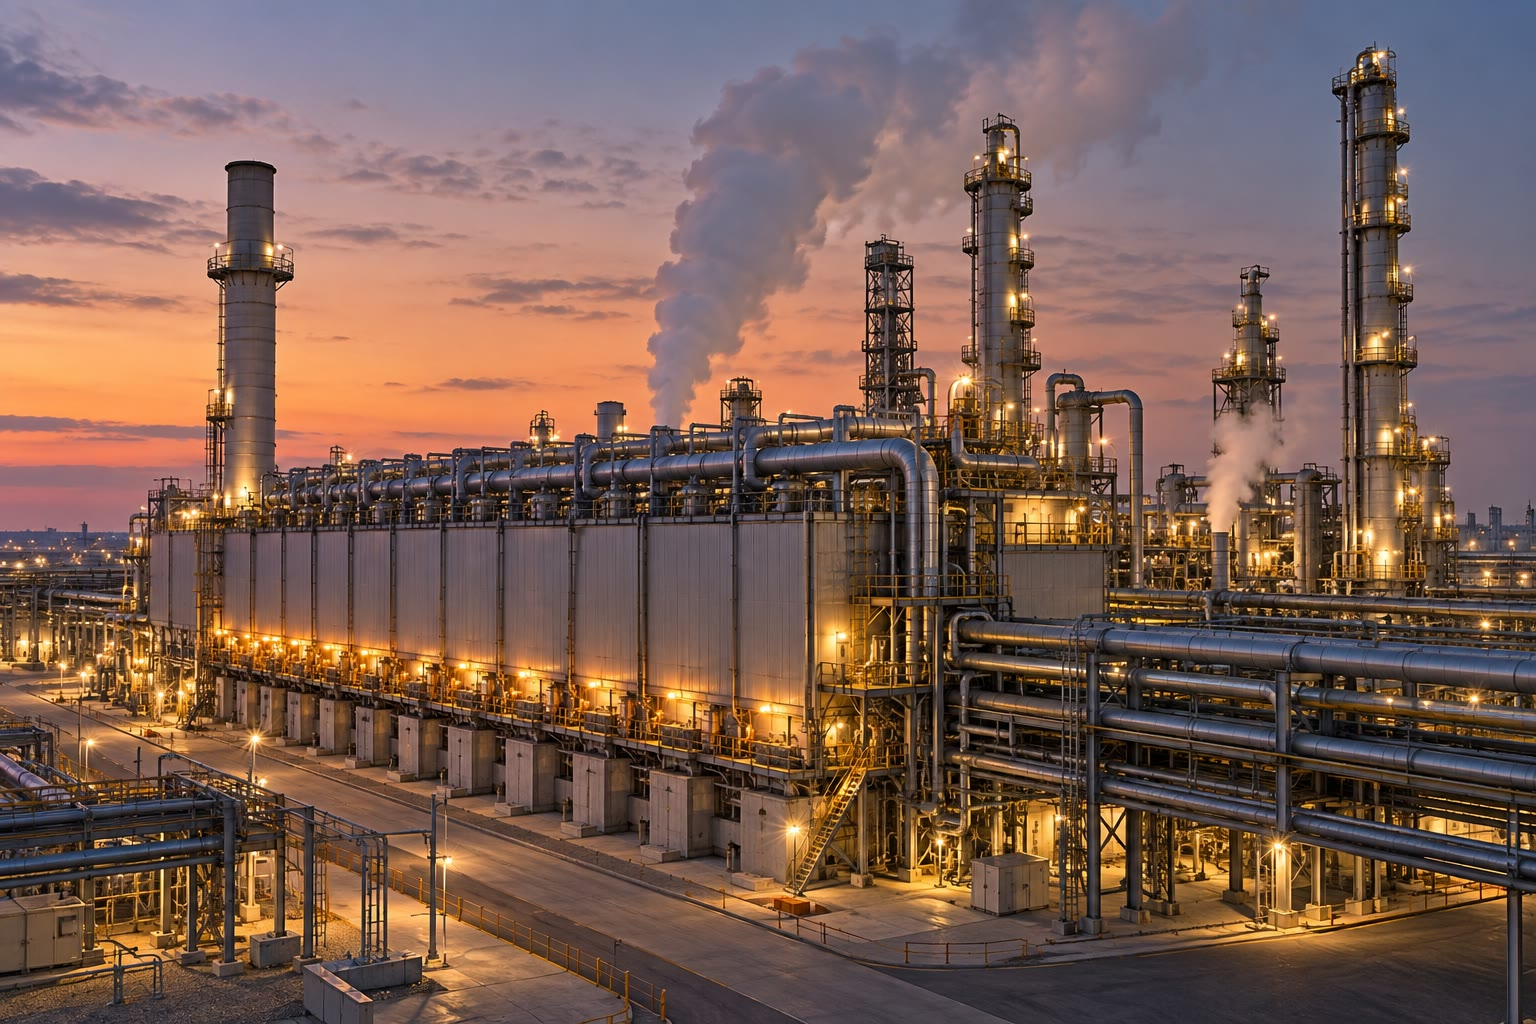
\includegraphics[width=0.6\linewidth]{images/book2/ai/b1-07-hydrogen-plant.jpg}

{\small Een waterstoffabriek in de schemering. Aardgas en stoom reageren
in de lange reformeroven; een tweede reactor zet koolstofmonoxide om; de
samenstelling aan de uitlaat is een eindtoestand van het soort dat in dit
hoofdstuk berekend wordt.}
\end{omfigure}

\section{Een systeem beschrijven}

\begin{definition}[Systeem, fase]\label{def:b1:extent-q-and-k:system}
Een \emph{fysisch-chemisch systeem}\index{fysisch-chemisch systeem} is de
materie in een gekozen gebied van de ruimte; de rest is zijn omgeving.
Het is een \emph{gesloten systeem}\index{gesloten systeem} als het geen
materie uitwisselt met de omgeving (energie mag wel). Een
\emph{fase}\index{fase} is een deel van het systeem waarin de \omterm{def:b1:extent-q-and-k:variables}{intensieve
grootheden} continu variëren: een gasmengsel is één fase, twee niet-mengbare
vloeistoffen zijn twee fasen, elke vaste stof is een fase op zich.
\end{definition}

\begin{definition}[Intensieve en extensieve grootheden]\label{def:b1:extent-q-and-k:variables}
Een toestandsgrootheid is \emph{extensief}\index{extensieve grootheid}
als ze evenredig is met de grootte van het systeem (massa, volume,
hoeveelheid stof) en \emph{intensief}\index{intensieve grootheid} als dat
niet zo is (temperatuur, druk, concentratie, dichtheid, \omterm{def:b1:extent-q-and-k:composition}{molfractie}). De
verhouding van twee extensieve grootheden is intensief.
\end{definition}

\begin{definition}[Samenstellingsgrootheden]\label{def:b1:extent-q-and-k:composition}
Voor een bestanddeel $i$ van een \omterm{def:b1:extent-q-and-k:system}{fase} die de hoeveelheden $n_j$ van al
haar bestanddelen bevat:
\begin{itemize}
  \item is zijn \emph{molfractie}\index{molfractie} $x_i = n_i/\sum_j
        n_j$, en zijn \emph{massafractie}\index{massafractie} $w_i =
        m_i/\sum_j m_j$; beide liggen tussen 0 en 1 en hebben als som 1;
  \item is zijn \emph{molaire
        concentratie}\index{molaire concentratie} in een oplossing met
        volume $V$ gelijk aan $c_i = [i] = n_i/V$,
        in \unit{mol/L};
  \item is zijn \emph{partiële
        druk}\index{partiele druk@partiële druk} in een gasmengsel met
        totale druk $p$ gelijk aan $p_i = x_i\,p$.
\end{itemize}
\end{definition}

\begin{proposition}[Partiële drukken van ideale gassen]\label{prop:b1:extent-q-and-k:dalton}
In een mengsel van ideale gassen met volume $V$ bij temperatuur $T$ is de
\omterm{def:b1:extent-q-and-k:composition}{partiële druk} van een bestanddeel de druk die het alleen in het hele
volume zou uitoefenen, $p_i = n_iRT/V$, en de \omterm{def:b1:extent-q-and-k:composition}{partiële drukken} tellen op
tot de totale druk: $\sum_i p_i = p$.
\end{proposition}

\begin{proof}
Voor het mengsel geldt $pV = (\sum_j n_j)RT$, dus $p_i = x_i p = \frac{n_i}{\sum_j
n_j}\cdot\frac{(\sum_j n_j)RT}{V} = \frac{n_iRT}{V}$, en $\sum_i x_i = 1$
geeft $\sum_i p_i = p$.
\end{proof}

\begin{example}[Lucht]\label{ex:b1:extent-q-and-k:air}
Droge lucht bevat, in volume (dus in hoeveelheid, voor ideale gassen),
78.08\,\% distikstof, 20.95\,\% dizuurstof en 0.93\,\% argon. Onder
\qty{1.013}{bar} is de \omterm{def:b1:extent-q-and-k:composition}{partiële druk} van dizuurstof $0.2095 \times
1.013 = \qty{0.212}{bar}$; op een berg waar de druk \qty{0.70}{bar} is,
daalt ze tot \qty{0.147}{bar}, hoewel de samenstelling dezelfde is.
% ledger: air:N2, air:O2, air:Ar, const:atm
\end{example}


\section{Reactievoortgang}

\begin{definition}[Stoichiometrische getallen, voortgang]\label{def:b1:extent-q-and-k:extent}
Een reactie wordt geschreven als $0 = \sum_i \nu_i\,\mathrm{A}_i$, waarin
het \emph{stoichiometrisch getal}\index{stoichiometrisch getal} $\nu_i$
van het deeltje $\mathrm{A}_i$ negatief is voor een beginstof en positief
voor een reactieproduct: in \ce{N2 + 3H2 -> 2NH3} is $\nu(\ce{N2}) = -1$,
$\nu(\ce{H2}) = -3$,
$\nu(\ce{NH3}) = +2$. In een \omterm{def:b1:extent-q-and-k:system}{gesloten systeem} waarin alleen deze reactie
plaatsvindt, veranderen de hoeveelheden volgens
\[
  n_i = n_{i,0} + \nu_i\,\xi ,
\]
wat de \emph{reactievoortgang}\index{reactievoortgang} $\xi$ definieert
(in mol), nul aan het begin en dezelfde voor elk deeltje.
\end{definition}

\begin{definition}[Maximale voortgang, beperkende beginstof]\label{def:b1:extent-q-and-k:max-extent}
De \emph{maximale voortgang}\index{maximale voortgang} $\xi_{\max}$ is de
grootste waarde van $\xi$ waarvoor geen enkele hoeveelheid negatief is:
$\xi_{\max} = \min_{\nu_i <
0} n_{i,0}/|\nu_i|$. De beginstof die bij $\xi_{\max}$ nul bereikt, is de
\emph{beperkende beginstof}\index{beperkende beginstof}. Wanneer de
voortgang ook negatief kan zijn (de omgekeerde reactie), is
$\xi_{\min} = -\min_{\nu_i > 0}
n_{i,0}/\nu_i$.
\end{definition}

\begin{method}[De voortgangstabel]\label{met:b1:extent-q-and-k:progress-table}
Zo volg je een reactie in een \omterm{def:b1:extent-q-and-k:system}{gesloten systeem}:
\begin{enumerate}
  \item schrijf de kloppende reactievergelijking op, met daaronder één
        kolom per deeltje;
  \item eerste rij: de beginhoeveelheden $n_{i,0}$;
  \item tweede rij: de hoeveelheden bij voortgang $\xi$, $n_{i,0} + \nu_i\xi$;
  \item voeg voor gassen een kolom toe met de totale hoeveelheid
        $n_{\text{tot}}(\xi)$;
  \item bereken $\xi_{\max}$ (en $\xi_{\min}$) en bepaal de \omterm{def:b1:extent-q-and-k:max-extent}{beperkende
        beginstof};
  \item laatste rij: de eindhoeveelheden, bij de eindvoortgang $\xi_f$
        (gevonden uit de evenwichtsvoorwaarde, of gelijk aan $\xi_{\max}$
        als de reactie aflopend is).
\end{enumerate}
\end{method}

\begin{example}[Synthese van ammoniak]\label{ex:b1:extent-q-and-k:ammonia}
Uitgaande van \qty{2.0}{mol} \ce{N2} en \qty{3.0}{mol} \ce{H2}:
\begin{center}
\begin{tabular}{lcccc}
\hline
 & \ce{N2} & \ce{3H2} & \ce{2NH3} & totaal \\
\hline
begin & 2.0 & 3.0 & 0 & 5.0 \\
voortgang $\xi$ & $2.0 - \xi$ & $3.0 - 3\xi$ & $2\xi$ & $5.0 - 2\xi$ \\
\hline
\end{tabular}
\end{center}
$\xi_{\max} = \min(2.0/1,\ 3.0/3) = \qty{1.0}{mol}$: diwaterstof is
beperkend. Als de reactie aflopend was, zou de eindtoestand
\qty{1.0}{mol} \ce{N2} en \qty{2.0}{mol} \ce{NH3} bevatten.
\end{example}

\begin{definition}[Omzettingsgraad, rendement]\label{def:b1:extent-q-and-k:fractional-extent}
De \emph{omzettingsgraad}\index{omzettingsgraad} van een reactie is
$\tau = \xi_f/\xi_{\max}$, tussen 0 en 1. In een synthese is het
\emph{rendement}\index{rendement} van een product de verhouding van de
verkregen hoeveelheid tot de hoeveelheid die de \omterm{def:b1:extent-q-and-k:max-extent}{beperkende beginstof} zou
opleveren als de reactie aflopend was; als er bij de isolatie geen
product verloren gaat, is het gelijk aan $\tau$.
\end{definition}

\section{Activiteiten}

\begin{definition}[Standaardtoestand, activiteit]\label{def:b1:extent-q-and-k:activity}
De \emph{activiteit}\index{activiteit} $a_i$ van een deeltje is een
dimensieloos getal dat in de uitdrukking van de evenwichtswetten meet
hoeveel ervan beschikbaar is; ze wordt gedefinieerd ten opzichte van een
\emph{standaardtoestand}\index{standaardtoestand}, een referentietoestand
bij de beschouwde temperatuur en onder de standaarddruk
$p^\circ = \qty{1}{bar}$. In de ideale benaderingen die in dit boek
gebruikt worden:
\begin{itemize}
  \item voor een gas is $a_i = p_i/p^\circ$ (de standaardtoestand is het
        zuivere ideale gas bij $p^\circ$);
  \item voor een opgeloste stof in een verdunde oplossing is
        $a_i = c_i/c^\circ$ met $c^\circ = \qty{1}{mol/L}$;
  \item voor het oplosmiddel van een verdunde oplossing, en voor een
        zuivere vaste stof of een zuivere vloeistof die alleen in haar \omterm{def:b1:extent-q-and-k:system}{fase}
        is, is $a_i = 1$.
\end{itemize}
\end{definition}
% ledger: const:pstd


\begin{remark}[Ideaal en reëel]\label{rem:b1:extent-q-and-k:ideal}
Deze uitdrukkingen gelden voor ideale gassen en voor verdunde
oplossingen. In geconcentreerde oplossingen trekken ionen elkaar aan en
stoten ze elkaar af, en wijkt de \omterm{def:b1:extent-q-and-k:activity}{activiteit} af van $c_i/c^\circ$; de
correcties, geschreven met activiteitscoëfficiënten, worden in het deel
van jaar 2 bestudeerd, samen met de chemische potentiaal. Voor de
concentraties die in dit boek gebruikt worden (onder ongeveer
\qty{0.1}{mol/L}) zijn de ideale uitdrukkingen tot op enkele procenten
nauwkeurig.
\end{remark}

\section{Het reactiequotiënt en de evenwichtsconstante}

\begin{definition}[Reactiequotiënt]\label{def:b1:extent-q-and-k:quotient}
Het \emph{reactiequotiënt}\index{reactiequotient@reactiequotiënt} van een
reactie $0 = \sum_i \nu_i\,\mathrm{A}_i$ in een gegeven toestand van het
systeem is
\[
  Q = \prod_i a_i^{\nu_i} ,
\]
het product van de \omterm{def:b1:extent-q-and-k:activity}{activiteiten} van de reactieproducten gedeeld door dat
van de beginstoffen, elk verheven tot de macht van zijn stoichiometrische
coëfficiënt.
\end{definition}

\begin{example}[Drie quotiënten]\label{ex:b1:extent-q-and-k:quotients}
Voor \ce{N2(g) + 3H2(g) <=> 2NH3(g)}: $Q = \dfrac{(p_{\ce{NH3}}/p^\circ)^2}
{(p_{\ce{N2}}/p^\circ)(p_{\ce{H2}}/p^\circ)^3}$. Voor
\ce{CH3COOH(aq) + H2O(l) <=> CH3COO^-(aq) + H3O+(aq)}: $Q =
\dfrac{[\ce{CH3COO-}][\ce{H3O+}]}{[\ce{CH3COOH}]\,c^\circ}$, waarbij het
oplosmiddel \omterm{def:b1:extent-q-and-k:activity}{activiteit} 1 heeft. Voor \ce{CaCO3(s) <=> CaO(s) + CO2(g)}:
$Q =
p_{\ce{CO2}}/p^\circ$, waarbij de vaste stoffen \omterm{def:b1:extent-q-and-k:activity}{activiteit} 1 hebben.
\end{example}

\begin{definition}[Standaardevenwichtsconstante]\label{def:b1:extent-q-and-k:equilibrium-constant}
De \emph{standaardevenwichtsconstante}\index{standaardevenwichtsconstante}
$K^\circ$ van een reactie is de waarde die haar \omterm{def:b1:extent-q-and-k:quotient}{reactiequotiënt} aanneemt
wanneer het systeem in evenwicht is. Ze is dimensieloos en hangt alleen
af van de reactie en de temperatuur.
\end{definition}

\begin{theorem}[Massawerkingswet]\label{thm:b1:extent-q-and-k:mass-action}
Bij een gegeven temperatuur evolueert een systeem waarin een reactie in
beide richtingen kan verlopen tot $Q = K^\circ(T)$; bij evenwicht geldt,
wat de beginsamenstelling ook is,
\[
  \prod_i a_{i,\text{eq}}^{\nu_i} = K^\circ(T) .
\]
\end{theorem}
\admitted

\begin{proposition}[Richting van de evolutie]\label{prop:b1:extent-q-and-k:direction}
Een systeem waarin $Q < K^\circ$ evolueert in voorwaartse richting
($\xi$ neemt toe); als $Q > K^\circ$, evolueert het in omgekeerde
richting; als $Q = K^\circ$, is het in evenwicht.
\end{proposition}
\admitted

\begin{remark}[Waar deze wetten vandaan komen]\label{rem:b1:extent-q-and-k:origin}
Beide uitspraken volgen uit de tweede hoofdwet van de thermodynamica, via
de vrije reactie-energie en de chemische potentialen van de deeltjes: ze
worden afgeleid in het deel van jaar 2, dat ook $K^\circ$ uit tabellen
van thermodynamische gegevens haalt en uitlegt hoe ze met de temperatuur
verandert. Hier worden ze als wetten gebruikt.
\end{remark}

\begin{omfigure}
\begin{tikzpicture}[font=\small, >={Stealth}]
  \draw[->, thick] (0,0) -- (11,0) node[right] {$Q$};
  \draw[thick, omThm] (5.5,0.25) -- (5.5,-0.25) node[below] {$K^\circ$};
  \draw[->, omDef, thick] (1.0,0.55) -- (4.6,0.55);
  \node[above, omDef] at (2.8,0.6) {$Q < K^\circ$: naar rechts};
  \draw[->, omProp, thick] (10.0,0.55) -- (6.4,0.55);
  \node[above, omProp] at (8.2,0.6) {$Q > K^\circ$: naar links};
  \node[below] at (0,-0.1) {0};
\end{tikzpicture}

{\small Het quotiënt beweegt naar de constante toe: een systeem met $Q <
K^\circ$ vormt reactieproducten, een systeem met $Q > K^\circ$ verbruikt
ze.}
\end{omfigure}

\begin{proposition}[Constanten combineren]\label{prop:b1:extent-q-and-k:combine-k}
Als $K_1^\circ$ en $K_2^\circ$ de constanten van de reacties (1) en (2)
zijn: de omgekeerde reactie van (1) heeft de constante $1/K_1^\circ$; de
reactie $n \times
(1)$ heeft $(K_1^\circ)^n$; de som $(1) + (2)$ heeft $K_1^\circ K_2^\circ$.
\end{proposition}

\begin{proof}
Het quotiënt van de omgekeerde reactie is $\prod a_i^{-\nu_i} = 1/Q_1$;
dat van $n \times (1)$ is $\prod a_i^{n\nu_i} = Q_1^n$; dat van de som is
$\prod a_i^{\nu_{i,1} + \nu_{i,2}} = Q_1 Q_2$. Deze identiteiten bij
evenwicht opschrijven, waar elk quotiënt gelijk is aan zijn constante,
geeft het resultaat.
\end{proof}

\begin{proposition}[Eén evenwichtstoestand]\label{prop:b1:extent-q-and-k:q-monotone}
Voor één enkele reactie in een \omterm{def:b1:extent-q-and-k:system}{gesloten systeem} bij vaste temperatuur
(en, voor gassen, bij vast volume of vaste druk) is het quotiënt $Q(\xi)$
een strikt stijgende functie van $\xi$ op $(\xi_{\min}, \xi_{\max})$, die
van 0 naar $+\infty$ gaat wanneer er geen deeltje met constante
\omterm{def:b1:extent-q-and-k:activity}{activiteit} bij betrokken is. De vergelijking $Q(\xi) = K^\circ$ heeft dan
precies één oplossing in dat interval.
\end{proposition}

\begin{proof}
Neem een reactie in oplossing, $Q(\xi) = \prod_i (n_{i,0} + \nu_i\xi)^{\nu_i}
\times \text{const}$. De logaritmische afgeleide is
\[
  \frac{\dd \ln Q}{\dd \xi} = \sum_i \frac{\nu_i^2}{n_{i,0} + \nu_i \xi}
  > 0 ,
\]
waarbij elke term positief is waar alle hoeveelheden het zijn. Als
$\xi \to \xi_{\max}$, gaat de hoeveelheid van een beginstof in een noemer
naar 0 en $Q \to +\infty$; als $\xi
\to \xi_{\min}$, gaat de hoeveelheid van een reactieproduct naar 0 en
$Q \to 0$. Een continue stijgende functie van 0 naar $+\infty$ neemt de
waarde $K^\circ$ één keer aan. (Voor gassen bij constante druk varieert
ook de totale hoeveelheid; het resultaat blijft gelden, wat in elk geval
afzonderlijk na te gaan is.)
\end{proof}

\section{Eindtoestanden}

\begin{definition}[Evenwichtstoestand, kwantitatieve reactie]\label{def:b1:extent-q-and-k:quantitative}
De eindtoestand is een \emph{evenwichtstoestand}\index{evenwichtstoestand}
wanneer alle deeltjes van de reactie aanwezig zijn en $Q = K^\circ$. De
reactie is \emph{kwantitatief}\index{kwantitatieve reactie} (of aflopend)
wanneer de \omterm{def:b1:extent-q-and-k:max-extent}{beperkende beginstof} in de eindtoestand praktisch verdwenen
is, $\xi_f \approx \xi_{\max}$; dat gebeurt wanneer $K^\circ$ zeer groot
is.
\end{definition}

\begin{method}[De eindtoestand bepalen]\label{met:b1:extent-q-and-k:final-state}
Zo bepaal je de eindtoestand van één enkele reactie:
\begin{enumerate}
  \item stel de voortgangstabel op en bereken $\xi_{\max}$ (en
        $\xi_{\min}$);
  \item bereken $Q$ aan het begin en vergelijk het met $K^\circ$ om de
        richting te vinden;
  \item druk $Q(\xi)$ uit met de \omterm{def:b1:extent-q-and-k:activity}{activiteiten} en los $Q(\xi) = K^\circ$ op
        naar $\xi$ in $(\xi_{\min}, \xi_{\max})$;
  \item is er een deeltje met \omterm{def:b1:extent-q-and-k:activity}{activiteit} 1 (een vaste stof) bij betrokken,
        controleer dan of het bij die voortgang nog aanwezig is: zou de
        hoeveelheid negatief moeten worden, dan verdwijnt het eerst en is
        de eindtoestand \emph{geen} evenwicht ($\xi_f = \xi_{\max}$,
        $Q_f \ne K^\circ$).
\end{enumerate}
\end{method}

\begin{method}[De hypothese van de kwantitatieve reactie]\label{met:b1:extent-q-and-k:quantitative}
Als $K^\circ$ groot is (typisch boven $10^4$), neem dan aan dat de
reactie aflopend is: stel $\xi_f = \xi_{\max}$, bereken de
eindhoeveelheden, en bepaal daarna de kleine hoeveelheid $\varepsilon$
van de \omterm{def:b1:extent-q-and-k:max-extent}{beperkende beginstof} die overblijft door $Q =
K^\circ$ te schrijven met de andere hoeveelheden ongewijzigd. De
hypothese wordt aanvaard als $\varepsilon$ klein is ten opzichte van de
andere hoeveelheden (onder ongeveer 1\,\%).
\end{method}

\begin{example}[Een kwantitatieve reactie]\label{ex:b1:extent-q-and-k:quant}
Voor $\mathrm{A + B \rightleftharpoons C + D}$ in oplossing met
$[\ce{A}]_0 = [\ce{B}]_0 =
\qty{0.10}{mol/L}$ en $K^\circ = 10^6$: in de veronderstelling dat de
reactie aflopend is, is $[\ce{C}]
= [\ce{D}] = 0.10$; dan geeft $0.10^2/\varepsilon^2 = 10^6$ de waarde
$\varepsilon
= \qty{1.0e-4}{mol/L}$, 0.1\,\% van de beginhoeveelheid: de hypothese is
gerechtvaardigd.
\end{example}

\begin{omfigure}
\begin{tikzpicture}
\begin{axis}[
  width=0.45\linewidth, height=5.6cm, ymode=log,
  xmin=0, xmax=1, ymin=0.01, ymax=1000,
  axis x line=bottom, axis y line=left,
  xlabel={voortgang $\xi$ (mol)}, ylabel={$Q$}, xtick={0,0.2,0.4,0.8,1},
  tick label style={font=\small}, label style={font=\small}, clip=false]
\addplot[omDef, thick] table[x=xi, y=Q] {figdata/out/bachelor-1-extent-equilibrium-shift.dat};
\draw[omThm, dashed] (axis cs:0,4) -- (axis cs:1,4);
\node[omThm, anchor=south west, font=\small] at (axis cs:0.02,4) {$K^\circ = 4.0$};
\draw[dotted] (axis cs:0.607,0.01) -- (axis cs:0.607,4);
\node[anchor=north, font=\small] at (axis cs:0.607,0.01) {0.607};
\end{axis}
\end{tikzpicture}\hfill
\begin{tikzpicture}
\begin{axis}[
  width=0.45\linewidth, height=5.6cm,
  xmin=0, xmax=0.04, ymin=0, ymax=0.3,
  axis x line=bottom, axis y line=left,
  xlabel={voortgang $\xi$ (mol)}, ylabel={$Q = p_{\ce{CO2}}/p^\circ$},
  xtick={0,0.01,0.02,0.03,0.04}, scaled x ticks=false,
  xticklabel style={/pgf/number format/fixed, /pgf/number format/precision=2},
  yticklabel style={/pgf/number format/fixed},
  tick label style={font=\small}, label style={font=\small}, clip=false]
\addplot[omProp, thick] table[x=xi, y=Q_small] {figdata/out/bachelor-1-extent-equilibrium-carbonate.dat};
\addplot[omDef, thick, dashed] table[x=xi, y=Q_large] {figdata/out/bachelor-1-extent-equilibrium-carbonate.dat};
\draw[omThm, dashed] (axis cs:0,0.2) -- (axis cs:0.04,0.2);
\node[omThm, anchor=south west, font=\small] at (axis cs:0.0005,0.2) {$K^\circ = 0.20$};
\node[omProp, anchor=north west, font=\scriptsize] at (axis cs:0.012,0.088) {\qty{0.010}{mol}: vaste stof op};
\node[omDef, anchor=north west, font=\scriptsize] at (axis cs:0.024,0.19) {\qty{0.050}{mol}: evenwicht};
\end{axis}
\end{tikzpicture}

{\small Links: het quotiënt van \ce{CO + H2O <=> CO2 + H2} stijgt met de
voortgang en bereikt $K^\circ$ één keer (weekendprobleem). Rechts: voor
\ce{CaCO3(s) <=> CaO(s) + CO2(g)} in een gesloten vat van \qty{10}{L}
groeit $Q = p_{\ce{CO2}}/p^\circ$ met $\xi$; met \qty{0.050}{mol}
carbonaat bereikt het $K^\circ = 0.20$ (evenwicht), met \qty{0.010}{mol}
is het carbonaat eerst op en is de eindtoestand geen evenwicht.}
\end{omfigure}

\begin{method}[Twee gelijktijdige reacties]\label{met:b1:extent-q-and-k:two-reactions}
Wanneer twee reacties in hetzelfde systeem plaatsvinden, geef dan elk zijn
eigen voortgang, $\xi_1$ en $\xi_2$; elke hoeveelheid is
$n_i = n_{i,0} + \nu_{i,1}\xi_1
+ \nu_{i,2}\xi_2$, en de eindtoestand voldoet zowel aan $Q_1 = K_1^\circ$
als aan
$Q_2 = K_2^\circ$ (een stelsel van twee vergelijkingen). Is de ene
constante veel groter dan de andere, behandel dan eerst de bijbehorende
reactie als \omterm{def:b1:extent-q-and-k:quantitative}{kwantitatief}, en daarna de tweede op het resultaat.
\end{method}

\begin{history}[De massawerkingswet, 1864]
In 1864 publiceerden de Noorse chemicus Cato Guldberg en zijn zwager, de
apotheker Peter Waage, in het Noors hun wet van de ``werkzame massa's'':
een reactie verloopt tot de krachten van de heen- en de teruggaande
reactie in evenwicht zijn, elk evenredig met de concentraties van haar
beginstoffen. Hun werk bleef in het buitenland onopgemerkt tot ze het in
twee meer gelezen talen opnieuw publiceerden, in 1867 en 1879; Jacobus
van 't Hoff, die de wet opnieuw had ontdekt, erkende hun voorrang.
\end{history}

\section{Oefeningen}

\begin{exercise}[$\star$]\label{exo:b1:extent-q-and-k:1}
Deel in als \omterm{def:b1:extent-q-and-k:variables}{intensief} of \omterm{def:b1:extent-q-and-k:variables}{extensief}: temperatuur, volume, hoeveelheid
stof, \omterm{def:b1:extent-q-and-k:composition}{molaire concentratie}, dichtheid, druk, massa, \omterm{def:b1:extent-q-and-k:composition}{molfractie}.
\end{exercise}

\begin{exercise}[$\star$]\label{exo:b1:extent-q-and-k:2}
Bereken met de samenstelling van droge lucht uit het hoofdstuk de
\omterm{def:b1:extent-q-and-k:composition}{partiële drukken} van \ce{N2}, \ce{O2} en \ce{Ar} onder een totale druk
van \qty{1.013}{bar}.
\end{exercise}

\begin{exercise}[$\star$]\label{exo:b1:extent-q-and-k:3}
Stel de voortgangstabel op van \ce{2H2 + O2 -> 2H2O} uitgaande van
\qty{3.0}{mol} \ce{H2} en \qty{2.0}{mol} \ce{O2}. Bepaal $\xi_{\max}$, de
\omterm{def:b1:extent-q-and-k:max-extent}{beperkende beginstof} en de eindtoestand als de reactie aflopend is.
\end{exercise}

\begin{exercise}[$\star$]\label{exo:b1:extent-q-and-k:4}
Schrijf het \omterm{def:b1:extent-q-and-k:quotient}{reactiequotiënt} op van: (a) \ce{CaCO3(s) <=> CaO(s) + CO2(g)};
(b) \ce{Ag+(aq) + Cl-(aq) <=> AgCl(s)}; (c) \ce{N2(g) + 3H2(g) <=>
2NH3(g)}; (d) \ce{NH3(aq) + H2O(l) <=> NH4+(aq) + OH-(aq)}.
\end{exercise}

\begin{exercise}[$\star\star$]\label{exo:b1:extent-q-and-k:5}
De reacties (1) $\mathrm{A \rightleftharpoons B}$ en (2) $\mathrm{B \rightleftharpoons C}$ hebben de constanten
$K_1^\circ = 10$ en $K_2^\circ = 0.5$. Geef de constanten van
$\mathrm{A \rightleftharpoons C}$,
$\mathrm{C \rightleftharpoons A}$ en $\mathrm{2\,A \rightleftharpoons 2\,C}$.
\end{exercise}

\begin{exercise}[$\star\star$]\label{exo:b1:extent-q-and-k:6}
Een reactie heeft $K^\circ = 2.0 \times 10^{-3}$. In welke richting
evolueert het systeem als aanvankelijk $Q = 5.0 \times 10^{-5}$? Als
$Q = 0.10$? Als er alleen beginstoffen aanwezig zijn?
\end{exercise}

\begin{exercise}[$\star\star$]\label{exo:b1:extent-q-and-k:7}
Het gas \ce{A2} dissocieert, \ce{A2(g) <=> 2A(g)}, met $K^\circ = 0.25$
bij de temperatuur van het experiment. Stel, uitgaande van
\qty{1.0}{mol} \ce{A2} onder een totale druk die op $p^\circ$ gehouden
wordt, de voortgangstabel op met de totale hoeveelheid, druk $Q(\xi)$ uit
en bepaal de evenwichtsvoortgang.
\end{exercise}

\begin{exercise}[$\star\star$]\label{exo:b1:extent-q-and-k:8}
In oplossing geldt $\mathrm{A + B \rightleftharpoons C}$ met $K^\circ = 100$ en de
beginconcentraties $[\ce{A}]_0 = [\ce{B}]_0 = \qty{0.10}{mol/L}$. Bepaal
de evenwichtsconcentraties en de \omterm{def:b1:extent-q-and-k:fractional-extent}{omzettingsgraad}.
\end{exercise}

\begin{exercise}[$\star\star$]\label{exo:b1:extent-q-and-k:9}
Toon voor $\mathrm{A + B \rightleftharpoons C + D}$, uitgaande van gelijke hoeveelheden \ce{A}
en \ce{B}, aan dat de \omterm{def:b1:extent-q-and-k:fractional-extent}{omzettingsgraad} $\tau = \sqrt{K^\circ}/(1 + \sqrt{K^\circ})$
is. Welke waarde van $K^\circ$ geeft $\tau = 0.99$?
\end{exercise}

\begin{exercise}[$\star\star\star$]\label{exo:b1:extent-q-and-k:10}
Calciumcarbonaat wordt bij \qty{1100}{K} verhit in een gesloten vat van
\qty{10.0}{L}, dat aanvankelijk geen gas bevat; voor
\ce{CaCO3(s) <=> CaO(s) + CO2(g)} is daar $K^\circ = 0.20$. Bepaal de
eindtoestand voor \qty{0.010}{mol} en voor \qty{0.050}{mol} carbonaat.
\end{exercise}

\begin{exercise}[$\star\star\star$]\label{exo:b1:extent-q-and-k:11}
Een stof \ce{A} isomeriseert in oplossing op twee manieren,
$\mathrm{A \rightleftharpoons B}$
($K_1^\circ = 2.0$) en $\mathrm{A \rightleftharpoons C}$ ($K_2^\circ = 3.0$). Bepaal, uitgaande
van \qty{1.0}{mol} \ce{A} alleen, de eindhoeveelheden van de drie
isomeren.
\end{exercise}

\begin{exercise}[$\star\star\star$]\label{exo:b1:extent-q-and-k:12}
Een zuur \ce{A} en een alcohol \ce{B} geven een ester en water, $\mathrm{A + B
\rightleftharpoons E + W}$, alles in één vloeibare \omterm{def:b1:extent-q-and-k:system}{fase}, met $K^\circ = 4.0$ (neem
de \omterm{def:b1:extent-q-and-k:activity}{activiteiten} gelijk aan de \omterm{def:b1:extent-q-and-k:composition}{molfracties}; de totale hoeveelheid
verandert niet). Bereken het maximale \omterm{def:b1:extent-q-and-k:fractional-extent}{rendement} aan ester uitgaande van
\qty{0.50}{mol} van elke beginstof, en daarna uitgaande van
\qty{0.50}{mol} zuur en \qty{1.0}{mol} alcohol.
\end{exercise}

\section{Probleem: de uitlaat van een waterstoffabriek}

\begin{problem}[{Weekendprobleem --- samenstellingsgrootheden van een
voeding, stoomreforming behandeld als aflopend, de watergasshiftreactie
in evenwicht, en het waterstofgehalte van het gas dat de fabriek
verlaat}]
\label{pb:b1:extent-q-and-k:1}
Een waterstoffabriek wordt gevoed met \qty{1.00}{mol} methaan en
\qty{3.00}{mol} stoom (per tijdseenheid) onder \qty{30}{bar}. In de
reformer wordt \ce{CH4 + H2O -> CO + 3H2} als aflopend beschouwd. In de
shiftreactor bereikt \ce{CO + H2O <=> CO2 + H2} evenwicht; neem
$K^\circ =
4.0$ bij zijn temperatuur. Molaire massa's: \ce{CH4} \qty{16.04}{g/mol},
\ce{H2O} \qty{18.02}{g/mol}.

\medskip
\noindent\textbf{Deel I --- De voeding.}
\begin{enumerate}
  \item Bereken de \omterm{def:b1:extent-q-and-k:composition}{molfracties} van methaan en stoom in de voeding.
  \item Bereken hun \omterm{def:b1:extent-q-and-k:composition}{partiële drukken}.
  \item Bereken hun \omterm{def:b1:extent-q-and-k:composition}{massafracties}.
  \item Welke van de tot nu toe gebruikte grootheden zijn \omterm{def:b1:extent-q-and-k:variables}{intensief}?
  \item Geef de \omterm{def:b1:extent-q-and-k:activity}{activiteiten} van methaan en stoom in de voeding.
\end{enumerate}

\medskip
\noindent\textbf{Deel II --- Reforming.}
\begin{enumerate}[resume]
  \item Stel de voortgangstabel van de reformingreactie op.
  \item Bereken $\xi_{\max}$ en noem de \omterm{def:b1:extent-q-and-k:max-extent}{beperkende beginstof}.
  \item Geef de hoeveelheden die de reformer verlaten.
  \item Bereken de totale hoeveelheid gas, en vergelijk met de voeding.
  \item Bereken de \omterm{def:b1:extent-q-and-k:composition}{molfracties} aan de uitlaat van de reformer.
  \item Waarom wordt stoom in overmaat toegevoerd?
\end{enumerate}

\medskip
\noindent\textbf{Deel III --- De shiftreactor.}
\begin{enumerate}[resume]
  \item Stel de voortgangstabel van de shiftreactie op, uitgaande van het
        gas dat de reformer verlaat.
  \item Toon aan dat $Q(\xi) = \dfrac{\xi(3 + \xi)}{(1 - \xi)(2 - \xi)}$, en
        dat het niet van de druk afhangt.
  \item Bereken $Q$ aan de inlaat en voorspel de richting van de
        evolutie.
  \item Schrijf de vergelijking voor de evenwichtsvoortgang op en los ze
        op, waarbij je de zinvolle wortel behoudt.
  \item Geef de hoeveelheden die de shiftreactor verlaten.
  \item Bereken de \omterm{def:b1:extent-q-and-k:fractional-extent}{omzettingsgraad} van de shiftreactie.
  \item Met twee keer zoveel stoom in de voeding (\qty{6.00}{mol}) komt het
        gas de shiftreactor binnen met \qty{5.00}{mol} stoom: bereken de
        nieuwe evenwichtsvoortgang.
\end{enumerate}

\medskip
\noindent\textbf{Deel IV --- Wat de fabriek verlaat.}
\begin{enumerate}[resume]
  \item Welke waarde van $K^\circ$ zou nodig zijn om in het eerste geval
        99\,\% van het koolstofmonoxide om te zetten?
  \item Leg uit waarom een shiftreactor meer omzet wanneer hij werkt bij
        een temperatuur waar zijn constante groter is, en waarom fabrieken
        twee shiftreactoren in serie gebruiken.
  \item De stoom wordt uit het gas dat de shiftreactor verlaat
        gecondenseerd. Bereken de \omterm{def:b1:extent-q-and-k:composition}{molfractie} waterstof in het droge gas.
  \item Som de onzuiverheden op die overblijven, met hun hoeveelheden.
  \item Bereken de \omterm{def:b1:extent-q-and-k:composition}{molfractie} waterstof in het gas dat de shiftreactor
        verlaat, stoom inbegrepen.
\end{enumerate}
\end{problem}
